\documentclass[pre,twocolumn,superscriptaddress,nofootinbib,longbibliography]{revtex4-2}

\usepackage{amsmath,amssymb,amsthm}
\usepackage{graphicx}
\usepackage{booktabs}
\usepackage[colorlinks=true,allcolors=blue]{hyperref}

\newtheorem{proposition}{Proposition}
\newtheorem{corollary}{Corollary}
\newcommand{\etaC}{\eta_{\mathrm{C}}}
\newcommand{\Pmax}{P_{\max}}
\newcommand{\todo}[1]{\textcolor{red}{[TODO: #1]}}

\begin{document}

\title{Efficiency or entropy production? Weighted-sum figures of merit miss most of the
Pareto front of quantum heat engines that saturate the thermodynamic uncertainty relation}

\author{Hugo Campos}
\affiliation{Universidad T\'ecnica Federico Santa Mar\'ia, Valpara\'iso, Chile}

\date{\today}

\begin{abstract}
Optimal cycles of microscopic heat engines are routinely found by maximizing a weighted sum of
power, efficiency (or entropy production) and power fluctuations, and the Pareto front is traced
by sweeping the weights. A weighted sum can only reach the supported part of a front, so whether
this procedure works depends on the front's geometry in the chosen objective coordinates. We show
that when the front saturates the thermodynamic uncertainty relation (TUR) and power and efficiency
can be tuned independently, it is a saddle surface in the coordinates (power, efficiency,
fluctuations): no interior point is reachable by any weighted sum. Rewritten with entropy
production instead of efficiency, the same surface becomes convex (though degenerate along rays),
and every point is reachable. For a finite-time Otto engine with a single qubit, whose front
saturates the TUR, $91\%$ of the front in efficiency coordinates is unsupported. A designer who
selects the cycle with a linear merit in efficiency reaches only $11\%$ of the front, and the best
reachable alternative is worse by a median of $14\%$ in at least one objective, with losses
concentrated in the low-noise, low-power regime. A linear merit in entropy production loses
nothing in the median. In the linear-response regime the front collapses to a curve and weighted
sums are exact, which reconciles our result with recent analytical fronts. Seven multi-objective
evolutionary algorithms confirm the picture: with efficiency as an objective, six of them exceed
the hypervolume ceiling of any weighted sum.
\end{abstract}

\maketitle

%=====================================================================
\section{Introduction}
%=====================================================================

A heat engine cannot be simultaneously powerful, efficient and reliable. For steady-state engines
this trade-off is quantified by the thermodynamic uncertainty relation
(TUR)~\cite{Barato2015,Gingrich2016}, which in the form of Pietzonka and
Seifert~\cite{Pietzonka2018} bounds the efficiency $\eta$ in terms of the mean power $P$ and the
power fluctuations $\Delta P$,
\begin{equation}
\eta \le \frac{\etaC}{1 + 2T_c P/\Delta P},
\label{eq:tur}
\end{equation}
with $\etaC = 1 - T_c/T_h$ the Carnot efficiency and $k_B = 1$. Related bounds trade power against
efficiency~\cite{Shiraishi2016}, and cyclic or periodically driven engines can evade or modify
Eq.~\eqref{eq:tur}~\cite{Holubec2018,Koyuk2019,Miller2021,Gramajo2023}.

Because these quantities compete, engine design is a multi-objective optimization problem whose
solution is a Pareto front rather than a single cycle. The most common way to compute such fronts
is to maximize a figure of merit that is a weighted sum of the normalized objectives and to sweep
the weights. Erdman \emph{et al.}~\cite{Erdman2023} used reinforcement learning to maximize
$F = aP/\Pmax - b\,\Delta P/\Delta P(\Pmax) - c\,\Sigma/\Sigma(\Pmax)$, with $\Sigma$ the entropy
production rate, and found that fast Otto cycles saturate the TUR. Almanza-Marrero, Rold\'an and
Manzano~\cite{Almanza2026} derived exact Pareto fronts in linear response by maximizing a weighted
sum that includes $\eta$ directly. Weighted sums are also the default in multi-objective
reinforcement learning~\cite{VanMoffaert2013} and in many applications of evolutionary
optimization to finite-time thermodynamics.

It is a classical result of multicriteria optimization that a weighted sum can only reach the
\emph{supported} points of a front, i.e., the points on its convex hull~\cite{DasDennis1997,Ehrgott2005}.
In stochastic thermodynamics this limitation has been noted for work fluctuations~\cite{Solon2018},
and nonconvex fronts have been reported when more control parameters are
released~\cite{Forao2025}. What has not been asked is how the shape of the front depends on
\emph{which} thermodynamic quantities are used as objectives. Efficiency and entropy production
are often treated as interchangeable, since at fixed power maximizing one minimizes the
other~\cite{Erdman2023}. For a weighted sum they are not interchangeable.

In this paper we show that the TUR fixes the geometry of the front. Our results are:
\begin{enumerate}
\item A proposition (Sec.~\ref{sec:geometry}): on a front that saturates Eq.~\eqref{eq:tur} and is
two-dimensional, the coordinates $(P,\eta,\Delta P)$ produce a saddle surface with no supported
interior point, whereas $(P,\Delta P,\Sigma)$ produce a convex, ruled surface on which every point is
supported.
\item A quantification of the physical cost for a finite-time single-qubit Otto engine
(Sec.~\ref{sec:otto}): the fraction of the front that a linear figure of merit can reach and how
much worse the best reachable cycle is.
\item The linear-response limit (Sec.~\ref{sec:lr}): the front of Ref.~\cite{Almanza2026} is a
curve on the TUR surface, fully supported, so the weighted sum there is exact.
\item A controlled comparison of seven multi-objective evolutionary algorithms (MOEAs) on two
models, with a decomposition of the hypervolume lost by the weighted sum into a part that no choice
of weights can recover and a part due to how the weights distribute solutions
(Secs.~\ref{sec:otto} and~\ref{sec:pw}).
\end{enumerate}

%=====================================================================
\section{Supported points and figures of merit}
\label{sec:supported}
%=====================================================================

We write all objectives as quantities to be minimized, $f = (f_1, f_2, f_3)$, e.g.,
$f = (-P, -\eta, \Delta P)$ or $f = (-P, \Delta P, \Sigma)$. A Pareto-optimal point $p$ of a front
$\mathcal{F}$ is \emph{supported} if there are weights $w \ge 0$, $\sum_i w_i = 1$, such that $p$
minimizes $w\cdot f$ over $\mathcal{F}$. Every maximizer of a figure of merit
$F = \sum_i a_i (\pm f_i)$ with nonnegative coefficients is supported, so the supported set is
exactly the set of cycles that a weighted-sum design can produce, for all weights. Supportedness
is invariant under positive affine rescaling of each objective, so the usual normalizations by
$\Pmax$, $\Delta P(\Pmax)$, etc., do not change it.

For a finite sample of the front we use the support gap~\cite{Ehrgott2005}
\begin{equation}
s^*(p) = \min_{w \ge 0,\ \sum w_i = 1}\ \max_{q \in \mathcal{F}}\ w\cdot\bigl(f(p) - f(q)\bigr),
\label{eq:gap}
\end{equation}
a linear program in $(w, s)$; $s^* = 0$ if and only if $p$ is supported, and $s^*>0$ measures, in
normalized units, how far $p$ is from being reachable. We call $p$ unsupported when
$s^* > 10^{-3}$ in coordinates normalized to the unit cube.

The gap is a geometric measure. To express the cost in physical terms, let $S$ be the supported
set of a given formulation and let $p$ be a point of the front in $(P,\eta,\Delta P)$. We define the
multiplicative loss
\begin{equation}
\varepsilon(p) = \min_{s \in S}\ \max\!\left(\frac{P_p}{P_s},\ \frac{\eta_p}{\eta_s},\
\frac{\Delta P_s}{\Delta P_p}\right) - 1 ,
\label{eq:eps}
\end{equation}
so that the best cycle a weighted-sum designer can obtain is at least a fraction $\varepsilon$
worse than $p$ in some physical objective.

%=====================================================================
\section{Geometry of TUR-saturating fronts}
\label{sec:geometry}
%=====================================================================

For heat engines with $0 < \eta < \etaC$ we use the entropy production rate
$\Sigma = Q_c/T_c - Q_h/T_h$ per unit time, which can be written as
\begin{equation}
\Sigma = \frac{P(\etaC - \eta)}{\eta\,T_c},
\qquad\text{equivalently}\qquad
\eta = \frac{\etaC P}{P + T_c\Sigma}.
\label{eq:sigma}
\end{equation}
In these variables the TUR reads $\Delta P\,\Sigma \ge 2P^2$, and the ratio
$\xi = 2P^2/(\Delta P\,\Sigma) = 2T_c P\eta/[\Delta P(\etaC-\eta)]$ satisfies $\xi \le 1$ for
steady-state engines, with equality at saturation.

\begin{proposition}
\label{prop}
Assume that (H1) the Pareto front saturates the TUR, $\Delta P = g(P,\eta) \equiv
2T_c\eta P/(\etaC - \eta)$, and (H2) it is a two-dimensional region of that surface, i.e., the graph
of $g$ over a set $D$ of $(P,\eta)$ with nonempty interior. Then:
\begin{enumerate}
\item[(i)] In coordinates $f = (-P,-\eta,\Delta P)$ no point with $(P,\eta)$ in the interior of $D$
is supported.
\item[(ii)] In coordinates $f = (-P, \Delta P, \Sigma)$ the same surface is the graph of
$h(P,\Sigma) = 2P^2/\Sigma$, which is convex. If the image $D'$ of $D$ in the $(P,\Sigma)$ plane is
convex, every point is supported, with nonnegative weights. The supporting weighted sums are
degenerate: each is minimized along a segment of a ray $P \propto \Sigma$.
\end{enumerate}
\end{proposition}

\begin{proof}
(i) Suppose $(P_0,\eta_0) \in \operatorname{int} D$ minimizes
$w_1(-P) + w_2(-\eta) + w_3 g(P,\eta)$. If $w_3 = 0$, a nonzero linear function would attain an
interior minimum, which is impossible; hence $w_3 > 0$, and the second-order necessary condition
requires $\nabla^2 g(P_0,\eta_0) \succeq 0$. But $g_{PP} = 0$ and
$g_{P\eta} = 2T_c\etaC/(\etaC - \eta)^2 \neq 0$, so
\begin{equation}
\det \nabla^2 g = -\frac{4T_c^2\etaC^2}{(\etaC - \eta)^4} < 0,
\end{equation}
and the Hessian is indefinite: the surface crosses its tangent plane at every interior point.
(ii) Substituting Eq.~\eqref{eq:sigma} gives $\Delta P = 2P^2/\Sigma$, the perspective of $2P^2$,
which is jointly convex for $\Sigma > 0$~\cite{Boyd2004}; its Hessian
$\tfrac{4}{\Sigma^3}\bigl(\begin{smallmatrix}\Sigma^2 & -P\Sigma\\ -P\Sigma & P^2\end{smallmatrix}\bigr)$
is positive semidefinite with null direction $(P,\Sigma)$. For convex $h$ on convex $D'$, the
tangent plane at any point supports the graph; the corresponding weights for
$(-P,\Delta P,\Sigma)$ are proportional to $(\partial_P h, 1, -\partial_\Sigma h) =
(4P/\Sigma, 1, 2P^2/\Sigma^2) \ge 0$. Since $h$ is positively homogeneous of degree one, it is
linear along rays, and the minimizer of the weighted sum is not unique along them.
\end{proof}

Two remarks. First, (H2) is essential: a curve lying on a saddle surface can be fully supported
(Sec.~\ref{sec:lr}). Second, the boundary of $D$ is not covered by part (i); in practice, supported
points of a TUR-saturating front in $(P,\eta,\Delta P)$ lie on parts of its boundary.
Figure~\ref{fig:geometry} shows a synthetic TUR-saturating surface with a hump-shaped domain
$0 < P \le \Pmax(\eta)$: $85\%$ of the points are unsupported in $(P,\eta,\Delta P)$ and none in
$(P,\Delta P,\Sigma)$.

\begin{figure}[t]
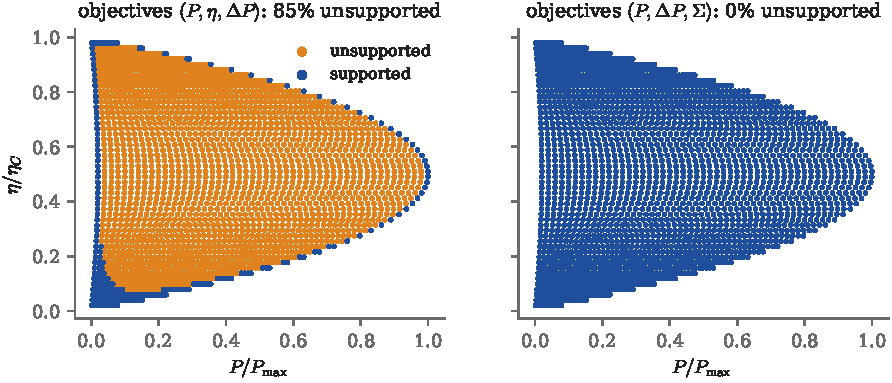
\includegraphics[width=\linewidth]{../figs/fig1_geometry.pdf}
\caption{A synthetic front that saturates the TUR ($\xi = 1$), $T_c = \etaC = 0.5$, $2500$ points,
classified by the support test~\eqref{eq:gap}. Left: objectives $(P,\eta,\Delta P)$; only boundary
points are supported. Right: the same cycles with objectives $(P,\Delta P,\Sigma)$; all points are
supported.}
\label{fig:geometry}
\end{figure}

\begin{corollary}
For engines satisfying (H1) and (H2), a figure of merit linear in $(P,\eta,\Delta P)$ cannot select
any cycle in the interior of the front, while a figure of merit linear in $(P,\Delta P,\Sigma)$
can select every cycle, up to the degeneracy along rays.
\end{corollary}

%=====================================================================
\section{Finite-time single-qubit Otto engine}
\label{sec:otto}
%=====================================================================

\subsection{Model and exact fluctuations}

The working medium is a two-level system with gap $\omega(t)$ ($\hbar = 1$), relevant for
superconducting-qubit engines~\cite{ErdmanNoe2022}. The cycle consists of (1) contact with a hot
bath at $T_h$ with gap $\omega_h$ for a time $\tau_h$; (2) a quench $\omega_h \to \omega_c$ of
duration $\tau_q$; (3) contact with a cold bath at $T_c$ with gap $\omega_c$ for a time $\tau_c$; and
(4) a quench back to $\omega_h$. Since the Hamiltonian commutes with itself at all times, no
coherences are generated and the qubit is a classical two-state Markov chain. During a bath
stroke the excited-state population relaxes as $p \to a + (p - a)e^{-\gamma\tau}$, with
$a = 1/(1+e^{\omega/T})$. The work extracted in one cycle is $w = (\omega_h - \omega_c)(s_1 - s_2)$,
with $s_1, s_2 \in \{0,1\}$ the states at the two quenches.

The full counting statistics follows from the tilted transfer matrix of one cycle,
$\mathcal{T}(\chi)_{ss'} = \sum_{s_1} M^h_{s s_1}e^{\chi\Delta\omega s_1}M^c_{s_1 s'}e^{-\chi\Delta\omega s'}$,
where $M^{h,c}$ are the relaxation matrices and $\Delta\omega = \omega_h - \omega_c$. The scaled
cumulant generating function is $\theta(\chi) = \ln\lambda_{\max}[\mathcal{T}(\chi)]$~\cite{Touchette2009},
and $P = \theta'(0)/\tau$, $\Delta P = \theta''(0)/\tau$, with
$\tau = \tau_h + \tau_c + 2\tau_q$. Because $\det\mathcal{T}(\chi) = e^{-\gamma(\tau_h+\tau_c)}$ does not
depend on $\chi$, $\lambda_{\max}$ has a closed form and both derivatives are analytic. The
efficiency is $\eta = 1 - \omega_c/\omega_h$ whenever $P > 0$, and $\Sigma$ follows from
Eq.~\eqref{eq:sigma}. We validated the expressions against Monte Carlo simulation of the jump
process and against finite differences of $\theta$.

We use $T_h = 1$, $T_c = 0.5$ ($\etaC = 0.5$), $\gamma = 1$ and $\tau_q = 0.05$. The four decision
variables are $\omega_h \in [0.1, 10]$, $r = \omega_c/\omega_h \in [T_c/T_h, 1]$ and
$\log_{10}\tau_{h,c} \in [-2, 1]$. At maximum power we find $\eta = 0.296$, close to the
Curzon--Ahlborn value $0.293$~\cite{CurzonAhlborn1975}.

\subsection{The front saturates the TUR}

A reference front was built from the union of a dense grid over the four variables and all
algorithm runs (Sec.~\ref{sec:algos}), and thinned on a voxel grid. Across the front the TUR ratio
has median $\xi = 0.996$ and maximum $1.005$ (Table~\ref{tab:otto}); the slight violations are
allowed for cyclic engines~\cite{Holubec2018}. This agrees with the saturation reported for fast
Otto cycles in Ref.~\cite{Erdman2023}. Power and efficiency are tuned independently through
$\omega_h$, $r$ and the stroke times, so the front fills a two-dimensional region
(Fig.~\ref{fig:lr}). Both hypotheses of Proposition~\ref{prop} hold.

As predicted, $91\%$ of the reference front is unsupported in $(P,\eta,\Delta P)$, with gaps up to
$0.077$, whereas only $4\%$ is unsupported in $(P,\Delta P,\Sigma)$, with gaps below $0.005$.

\subsection{Physical cost of a linear figure of merit}

Figure~\ref{fig:cost} maps the loss~\eqref{eq:eps} over the front in the $(P,\eta)$ plane. A
designer who maximizes a merit linear in $(P,\eta,\Delta P)$ can reach $11\%$ of the front. For
the rest, the best reachable cycle is worse by a median of $14\%$ in at least one objective;
$75\%$ of the front has $\varepsilon > 5\%$ and $60\%$ has $\varepsilon > 10\%$. The losses
concentrate at low power and intermediate to high efficiency (median $P/\Pmax = 0.34$,
$\eta/\etaC = 0.68$ among points with $\varepsilon > 5\%$): the low-noise cycles that matter for
precise operation. In the most extreme case, a cycle with $P/\Pmax = 0.075$ and
$\eta/\etaC = 0.55$ has, as its best reachable alternative, a cycle with $\eta/\etaC = 0.24$ and
$2.3$ times its fluctuations.

A merit linear in $(P,\Delta P,\Sigma)$, evaluated on the same physical cycles, reaches $98\%$ of
its front; the median loss over the $(P,\eta,\Delta P)$ front is zero, and only $7\%$ of it has
$\varepsilon > 5\%$. Writing the figure of merit with $\Sigma$, as in Ref.~\cite{Erdman2023},
therefore recovers almost the whole efficiency front.

\begin{figure*}[t]
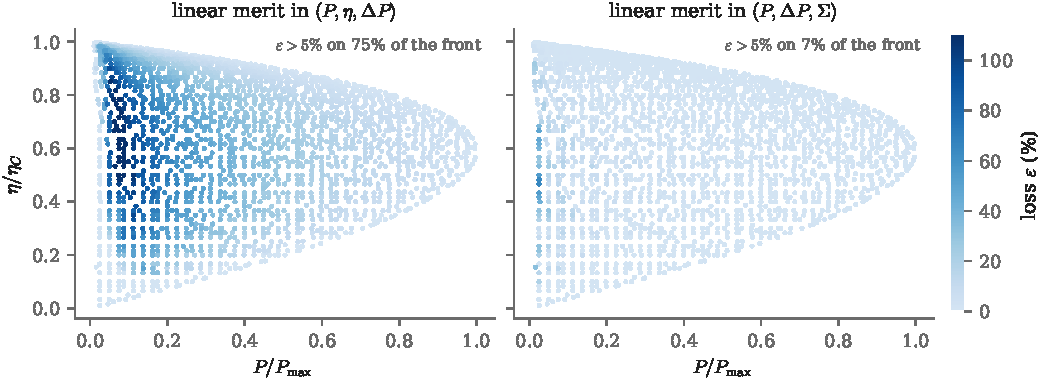
\includegraphics[width=0.9\linewidth]{../figs/fig2_cost.pdf}
\caption{Physical cost of designing the Otto engine with a linear figure of merit. Each point is a
cycle of the Pareto front in $(P,\eta,\Delta P)$, colored by the loss $\varepsilon$ of
Eq.~\eqref{eq:eps}: the best cycle reachable by any weighted sum is at least $\varepsilon$ worse in
some objective. Left: merit linear in $(P,\eta,\Delta P)$. Right: merit linear in
$(P,\Delta P,\Sigma)$.}
\label{fig:cost}
\end{figure*}

\subsection{Multi-objective evolutionary algorithms}
\label{sec:algos}

We compared seven MOEAs with the same budget: NSGA-II~\cite{Deb2002}, NSGA-III~\cite{DebJain2014},
SMS-EMOA~\cite{Beume2007}, RVEA~\cite{Cheng2016}, MOEA/D with normalized Tchebycheff
scalarization~\cite{ZhangLi2007}, MOEA/D with the adaptive weight adjustment of Qi
\emph{et al.} (MOEA/D-AWA)~\cite{Qi2014}, and MOEA/D with a linear weighted-sum scalarization
(MOEA/D-WS). The last one is the evolutionary counterpart of a weighted-sum design with $105$
uniformly spread weight vectors. Settings and the statistical protocol are given in
Appendix~\ref{app:protocol}.

To separate the two reasons why a weighted sum can lose hypervolume (HV)~\cite{Zitzler1999}, we
compute the HV of the supported points of the reference front. This is the \emph{ceiling} of any
weighted-sum method, whatever its weights. The gap between the reference HV and this ceiling is
the \emph{reachability} loss; the gap between the ceiling and the HV obtained by MOEA/D-WS is the
\emph{distribution} loss.

\begin{table}[t]
\caption{Otto engine, $30$ seeds, $42\,000$ evaluations per run. Median HV (reference point $1.1$
in normalized coordinates). All differences with respect to MOEA/D-AWA are significant
($p = 1.8\times10^{-10}$, Mann--Whitney with Holm correction).}
\label{tab:otto}
\begin{ruledtabular}
\footnotesize
\begin{tabular}{lcc}
 & $(P,\eta,\Delta P)$ & $(P,\Delta P,\Sigma)$ \\
\hline
TUR ratio $\xi$ (median / max) & 0.996 / 1.005 & 0.990 / 1.005 \\
Unsupported (max gap) & 91\% (0.077) & 4\% (0.005) \\
HV reference front & 1.0810 & 1.2114 \\
HV ceiling, any weighted sum & \textbf{0.9950} & 1.2113 \\
\hline
SMS-EMOA & 1.0425 & 1.1868 \\
MOEA/D-AWA & 1.0404 & 1.1829 \\
MOEA/D (Tchebycheff) & 1.0385 & 1.1744 \\
NSGA-III & 1.0310 & 1.1700 \\
RVEA & 1.0269 & 1.1683 \\
NSGA-II & 1.0073 & 1.1612 \\
MOEA/D-WS & 0.9670 & 1.1220 \\
\hline
WS loss: reach.\ + distr. & \textbf{0.086} + 0.028 & 0.0001 + \textbf{0.089}
\end{tabular}
\end{ruledtabular}
\end{table}

Table~\ref{tab:otto} and Fig.~\ref{fig:hv} show the result. MOEA/D-WS is last in both
formulations and loses a similar amount of HV, but for different reasons. With $\eta$ as an
objective, most of the loss is reachability: no choice of weights can recover it, and six of the
seven algorithms, including NSGA-II, exceed the ceiling of any weighted sum. With $\Sigma$, the
reachability loss vanishes and the whole deficit is distribution: MOEA/D-WS returns only $68$
distinct solutions out of $105$ because its optima pile up along the degenerate rays of
Proposition~\ref{prop}(ii). This part could in principle be recovered by better-placed weights;
the reachability loss in $\eta$ cannot. Among the algorithms that do not rely on a linear
scalarization, SMS-EMOA attains the highest HV and MOEA/D-AWA the lowest IGD+~\cite{Ishibuchi2015}
in both formulations (Appendix~\ref{app:protocol}).

\begin{figure*}[t]
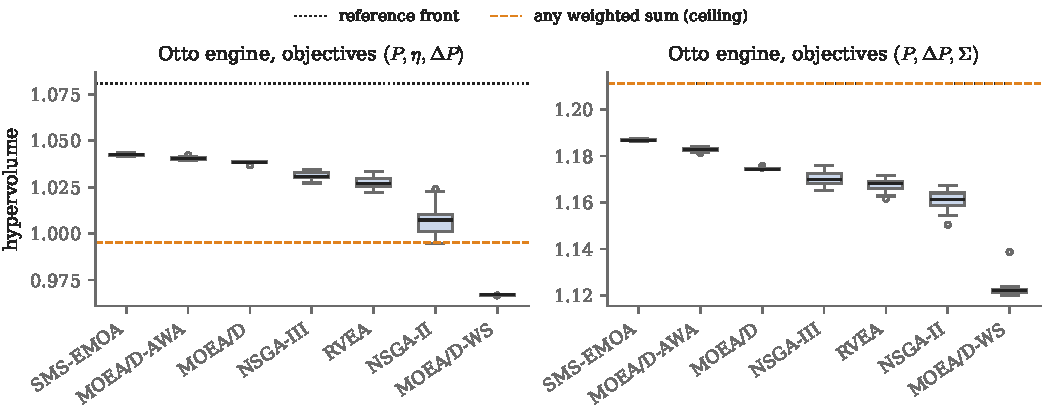
\includegraphics[width=0.9\linewidth]{../figs/fig3_hv_otto.pdf}
\caption{Hypervolume of seven MOEAs on the Otto engine ($30$ seeds). Dotted: reference front.
Dashed: HV of the supported part of the reference front, the ceiling of any weighted-sum method.
In $(P,\eta,\Delta P)$ (left) the ceiling lies below six of the seven algorithms; in
$(P,\Delta P,\Sigma)$ (right) it coincides with the reference front.}
\label{fig:hv}
\end{figure*}

%=====================================================================
\section{The linear-response limit}
\label{sec:lr}
%=====================================================================

Almanza-Marrero \emph{et al.}~\cite{Almanza2026} obtained exact fronts for machines in linear
response by maximizing
$\Omega = \alpha\bar P + \beta\bar\eta - \gamma\bar\Sigma - (1-\alpha-\beta-\gamma)\bar\sigma_P^2$,
a weighted sum that includes the efficiency. Proposition~\ref{prop} does not contradict their
result, because their front violates (H2).

With Onsager coefficients $L_{12} = q\sqrt{L_{11}L_{22}}$, fixed resources $A_2 = L_{22} = T = 1$
and the notation of Ref.~\cite{Almanza2026}, all objectives depend on the design variables only
through $y = \sqrt{L_{11}}A_1$ and $q$:
\begin{gather}
P = -y(y+q),\qquad \bar\eta = \frac{-y(y+q)}{1+qy},\nonumber\\
\Sigma = 1 + 2qy + y^2,\qquad \sigma_P^2 = 2y^2 .
\end{gather}
For fixed $y$, tight coupling $q = 1$ increases $P$ and $\bar\eta$ and decreases $\Sigma$, so the
front is the endoreversible family. With $e = -y \in [0,1]$,
\begin{equation}
P = e(1-e),\quad \bar\eta = e,\quad \Sigma = (1-e)^2,\quad \sigma_P^2 = 2e^2,
\end{equation}
a one-parameter curve with $P = 4\Pmax\bar\eta(1-\bar\eta)$ that saturates the TUR exactly,
$\sigma_P^2\Sigma = 2P^2$. A curve on a saddle can be fully supported, and this one is: maximizing
$\Omega$ over $e$ is a concave quadratic problem whose maximizer covers $[0,1]$ as the weights vary,
reproducing Eqs.~(7)--(10) of Ref.~\cite{Almanza2026}.

We verified this numerically with $2\times10^5$ random designs $(A_1, L_{11}, q)$: $99.95\%$ of the
nondominated designs have $q = 1$ (the rest have $q \to 1$), the front deviates from the analytic
curve by at most $2\times10^{-5}$, and the support test finds no unsupported point in
$(P,\eta,\Sigma,\sigma_P^2)$ or in any three-objective subset.

The contrast with the finite-time Otto engine is shown in Fig.~\ref{fig:lr}. In linear response
there is a single effective degree of freedom, so power and efficiency are locked together and the
weighted sum is exact. Beyond linear response, power and efficiency decouple, the front gains a
dimension, and, if it still saturates the TUR, the weighted sum in efficiency misses most of it.
Note that the two fronts are normalized by their own $\Pmax$; the figure compares dimensionality,
not bounds.

\begin{figure}[t]
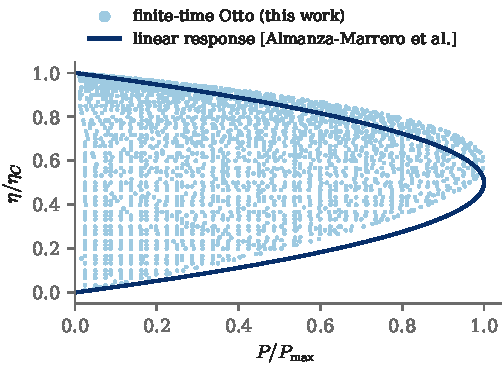
\includegraphics[width=\linewidth]{../figs/fig4_linear_response.pdf}
\caption{Pareto front of the finite-time Otto engine projected on the $(P,\eta)$ plane (points),
and the linear-response front of Ref.~\cite{Almanza2026} (line). The former is two-dimensional,
the latter a curve. Each is normalized by its own maximum power.}
\label{fig:lr}
\end{figure}

%=====================================================================
\section{Beyond TUR saturation: piecewise control}
\label{sec:pw}
%=====================================================================

To test what happens when (H1) fails, we used the quantum-dot engine of Erdman
\emph{et al.}~\cite{Erdman2023}, $H(t) = u(t)E_0\sigma_z/2$ with relaxation
$\dot p = -\gamma[p - f(\beta(t)E_0u(t))]$, $f(x) = 1/(1+e^x)$, $\beta_H = 1$, $\beta_C = 2$,
$E_0 = 2.5$, $u \in [0.2, 1.1]$ and $\gamma = 1$. The cycle of duration $\tau$ is split into $N = 8$
equal steps, each with its own $u_k$ and bath, giving $17$ decision variables. Exact statistics
follow from the product of tilted step matrices, as in Sec.~\ref{sec:otto}; the model reproduces
the four-variable Otto engine to $10^{-9}$ when restricted to it.

With free control the front violates the stationary TUR strongly: $81\%$ of the reference front
has $\xi > 1$, with $\xi$ up to $4.0$ (median $1.45$ in $\Sigma$ coordinates and $1.59$ in $\eta$
coordinates). Here the saddle disappears. Although $31\%$ ($\Sigma$) and $48\%$ ($\eta$) of the
reference front fail the support test at tolerance $10^{-3}$, the gaps are small (median about
$0.003$) and the ceiling of any weighted sum lies within $0.1\%$ ($\Sigma$) and $0.2\%$ ($\eta$) of
the reference HV (Table~\ref{tab:pw}). The front is nearly convex in both coordinate systems.

\begin{table}[t]
\caption{Piecewise control ($N = 8$, $17$ variables), $30$ seeds, $315\,000$ evaluations per run.
Median HV; $p$-values for MOEA/D-WS vs MOEA/D-AWA (Mann--Whitney, Holm).}
\label{tab:pw}
\begin{ruledtabular}
\footnotesize
\begin{tabular}{lcc}
 & $(P,\eta,\Delta P)$ & $(P,\Delta P,\Sigma)$ \\
\hline
TUR ratio $\xi$ (median / max) & 1.59 / 4.04 & 1.45 / 4.02 \\
HV reference / ceiling & 1.1208 / 1.1184 & 1.2284 / 1.2276 \\
SMS-EMOA & 1.0846 & 1.2094 \\
MOEA/D-AWA & 1.0654 & 1.1867 \\
MOEA/D-WS & 1.0586 ($p = 0.017$) & 1.1929 ($p = 0.011$) \\
WS loss: reach. + distr. & 0.0024 + 0.060 & 0.0008 + 0.035
\end{tabular}
\end{ruledtabular}
\end{table}

MOEA/D-WS still does worse relative to MOEA/D-AWA in $\eta$ than in $\Sigma$ coordinates, where it
is second only to SMS-EMOA (Fig.~\ref{fig:pw}). But its losses are now entirely distribution
losses, which Proposition~\ref{prop} does not address. The geometric effect is therefore tied to
TUR saturation: strong for the Otto engine, where the reachability loss is $8\%$ of the reference
HV, and negligible when free control breaks the bound.

\begin{figure*}[t]
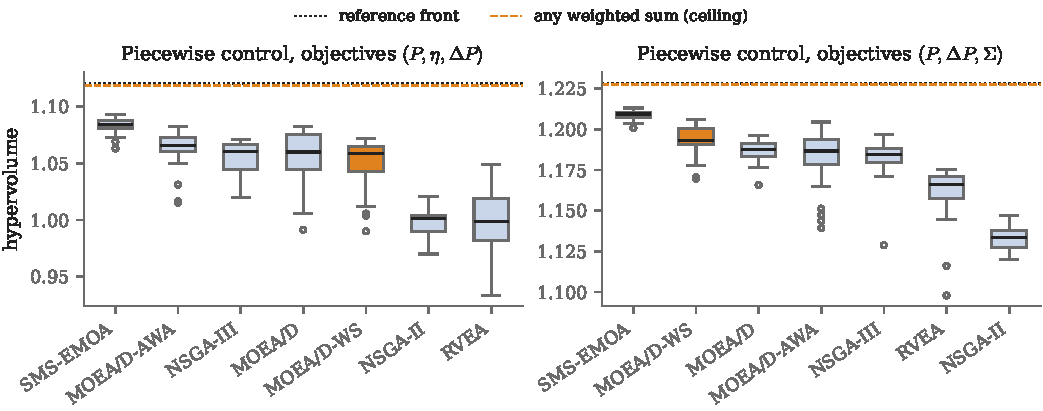
\includegraphics[width=0.9\linewidth]{../figs/fig5_hv_piecewise.pdf}
\caption{Hypervolume of seven MOEAs on the piecewise-controlled quantum-dot engine ($30$ seeds).
Lines as in Fig.~\ref{fig:hv}. The ceiling of any weighted sum is close to the reference front in
both formulations.}
\label{fig:pw}
\end{figure*}

%=====================================================================
\section{Discussion}
\label{sec:discussion}
%=====================================================================

Our results give a simple rule for practitioners: when an engine operates near TUR saturation,
a linear figure of merit should be written with the entropy production, not the efficiency. The
two are often treated as interchangeable because at fixed power they are monotonically
related, Eq.~\eqref{eq:sigma}, but the nonlinear map between them turns a convex surface into a
saddle. If efficiency must appear explicitly, the weighted sum should be replaced by a
nonlinear scalarization (e.g., Tchebycheff) or by a dominance- or indicator-based method; all of
these exceeded the weighted-sum ceiling in our Otto benchmark.

The condition is not exotic. TUR saturation has been reported for fast-driven Otto
cycles~\cite{Erdman2023}, and the Otto engine of Sec.~\ref{sec:otto} saturates it over its whole
front. Conversely, the linear-response fronts of Ref.~\cite{Almanza2026} saturate the TUR but are
one-dimensional, so weighted sums are exact there. The problem appears precisely in the regime
that motivates numerical optimization in the first place: far from equilibrium, with several
independent controls.

Several limitations should be noted. Our engines are classical stochastic models without
coherences; quantum friction and coherent driving can push fluctuations below the classical
TUR~\cite{Miller2021,Gramajo2023}, and the geometry of such fronts remains to be studied. The
support test is applied to a discrete reference front, so the ceiling is an estimate with an
error of the order of the tolerance. Finally, for engines that violate the TUR by a bounded
factor, it is an open question how the reachability loss interpolates between the saturated case
($\xi = 1$, large loss) and the piecewise case ($\xi$ up to $4$, negligible loss).

%=====================================================================
\section{Conclusions}
%=====================================================================

We proved that the Pareto front of an engine saturating the TUR is a saddle in
$(P,\eta,\Delta P)$ and a convex, ruled surface in $(P,\Delta P,\Sigma)$, provided power and
efficiency can be varied independently. For a finite-time qubit Otto engine, a weighted-sum design
with efficiency reaches $11\%$ of the front and loses a median of $14\%$ in some objective, whereas
the same design with entropy production loses nothing in the median. In linear response the front
is a curve and weighted sums are exact; under free piecewise control the bound is broken and the
front is nearly convex. The choice between efficiency and entropy production is therefore not a
matter of taste: it decides which engines a weighted-sum design can find.

\begin{acknowledgments}
\todo{Acknowledgments and funding.}
\end{acknowledgments}

\section*{Data availability}
\todo{Code and data: repository link.} All results can be reproduced with the scripts listed in
the repository README.

\appendix

\section{Algorithms and statistical protocol}
\label{app:protocol}

All algorithms use population size $N = 105$ (Das--Dennis weights with $13$ divisions for three
objectives), simulated binary crossover (probability $1$, $\eta_c = 20$) and polynomial mutation
($\eta_m = 20$). The pymoo~0.6.2 implementations~\cite{Blank2020} were used for NSGA-II, NSGA-III,
SMS-EMOA and RVEA. MOEA/D, MOEA/D-AWA and MOEA/D-WS share our implementation: neighborhood size
$10\%$ of $N$, mating from the neighborhood with probability $\delta = 0.9$, at most $n_r = 2$
replacements, and objectives normalized by the current ideal and nadir points. MOEA/D-AWA follows
Ref.~\cite{Qi2014}: the WS-transformation of the weights, an external population of size $1.5N$
truncated by sparsity (product of distances to the $m$ nearest neighbors), adjustment of $5\%$ of
the weights every $10$ generations after $80\%$ of the run.

The budgets are $400$ generations ($42\,000$ evaluations) for the Otto engine and $3000$
generations ($315\,000$ evaluations) for the piecewise model, with $30$ seeds per algorithm and
formulation. Reference fronts are the nondominated union of all runs, plus a dense grid sweep of
the four variables (Otto) or five additional long SMS-EMOA runs (piecewise), thinned on a
$60^3$ voxel grid. HV uses reference point $1.1$ in coordinates normalized by the reference
front; IGD+ is computed against the reference front. Each algorithm is compared with MOEA/D-AWA
by a two-sided Mann--Whitney test with Holm correction over six comparisons~\cite{Holm1979}.

\begin{table}[h]
\caption{Median IGD+ (lower is better).}
\setlength{\tabcolsep}{3pt}
\label{tab:igd}
\begin{ruledtabular}
\scriptsize
\begin{tabular}{lcccc}
 & \multicolumn{2}{c}{Otto} & \multicolumn{2}{c}{Piecewise} \\
 & $\eta$ & $\Sigma$ & $\eta$ & $\Sigma$ \\
\hline
SMS-EMOA & 0.0276 & 0.0183 & 0.0243 & 0.0151 \\
MOEA/D-AWA & 0.0198 & 0.0142 & 0.0266 & 0.0195 \\
MOEA/D & 0.0251 & 0.0220 & 0.0257 & 0.0182 \\
NSGA-III & 0.0252 & 0.0227 & 0.0289 & 0.0188 \\
RVEA & 0.0277 & 0.0224 & 0.0478 & 0.0230 \\
NSGA-II & 0.0380 & 0.0275 & 0.0664 & 0.0664 \\
MOEA/D-WS & 0.0745 & 0.0664 & 0.0323 & 0.0194
\end{tabular}
\end{ruledtabular}
\end{table}

\bibliography{refs}

\end{document}
